\chapter{Application in a serious Game}
In the course of the last chapters of this seminar work, many techniques to convey a desired atmosphere have been talked about and presented. Therefore, some applications of these techniques will now be illustrated by a real example. A serious game, which was also developed in the context of this seminar paper, will serve as an illustrative object. \\

The underlying game represents a serious game. Serious games are computer games whose main objective is not the pure entertainment of the player, but rather a therapeutic, educational or didactic value \cite{serious}. The serious game shown here aims to be used in the therapy of the hoarding disorder. \\\\
In short, the game is used to confront a patient with an unorganized, dirty apartment. He is then asked to tidy it up bit by bit. Initially, the atmosphere of the game scene, i.e. his virtual apartment, is supposed to appear very grim and dystopian. In the course of the game, the more the player brings order to the scene, the more pleasant and lighter the atmosphere should become. This effect is mainly created by some applications through above mentioned scene lighting techniques. The game itself was developed by a student team at Kempten University of Applied Sciences in cooperation with the "vfkv - Ausbildungsinstitut München gGmbH". The goal was to use the game to accompany during therapy under the supervision of a therapist.
\begin{figure}[H]
	\centering
		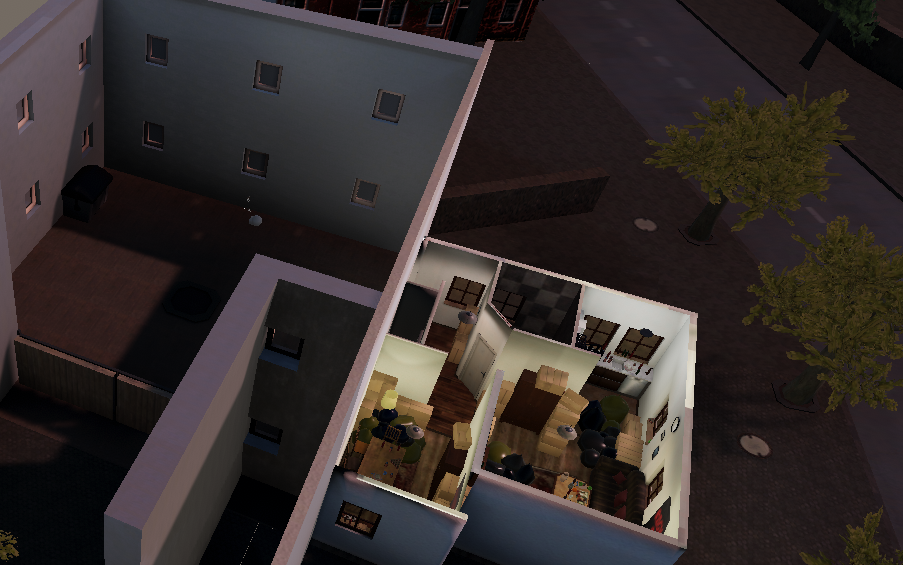
\includegraphics[width=0.7\textwidth]{Bilder/Erfassen.PNG}
	\caption{The game is divided into two scenes. The apartment and a courtyard. }
	\label{fig:szenes}
\end{figure}
\newpage
At first, the player stands in a courtyard to his virtual apartment. He sees a door, which is illuminated with a light directly above it. Although the light is not extremely strong, it already represents a key light, which draws attention to this door. This establishes it as a point of interest for the player. Since it is used to start the therapy, this effect is also very intentional. \\

\begin{figure}[H]
	\centering
		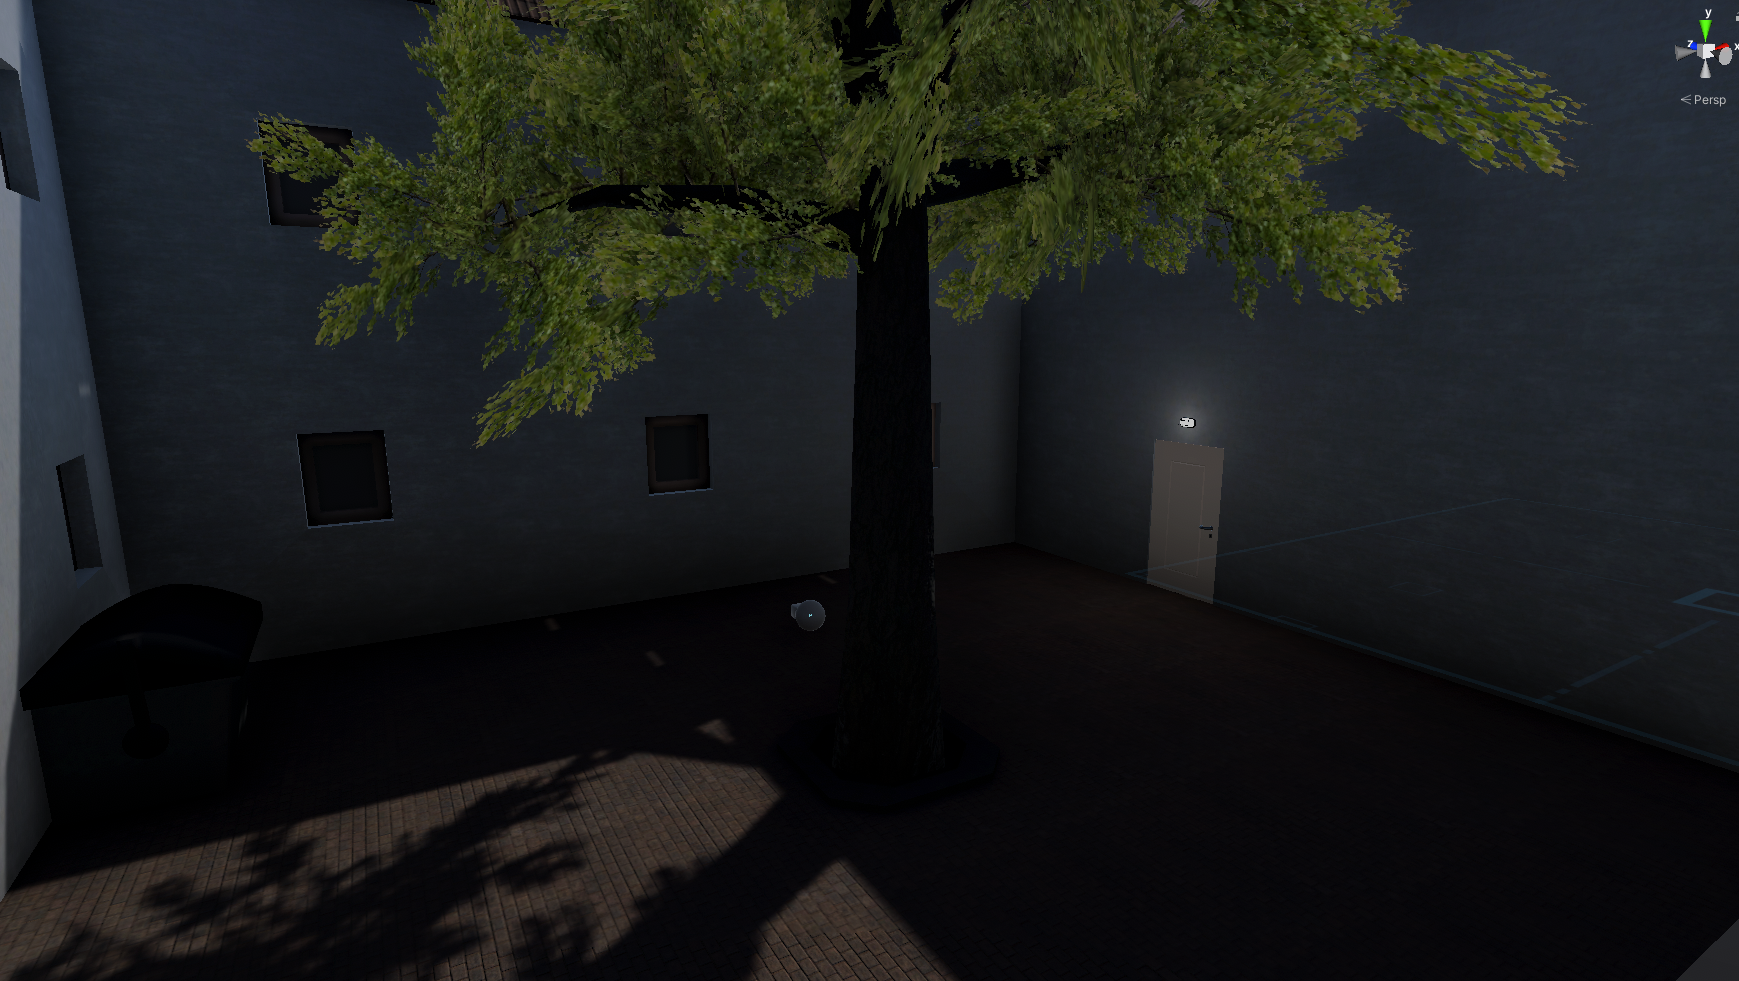
\includegraphics[width=0.7\textwidth]{Bilder/Innenhof keylight.PNG}
	\caption{The courtyard and a the door with a keylight above it. }
	\label{fig:door}
\end{figure}


The therapist, which can influence the gameplay at all times, has the possibility to give the player visual hints on how to navigate the level. These visual hints are described further in section \ref{chap:witcher} of this paper. \\
In addition, the therapist can add a yellow rim to objects that the player should interact with. This not only guides the player to this object, but also represents a rim light and hits implications made in the previous chapters (see chapter \ref{chapter:ThreePoint}). The yellow border makes the object stand out very strongly from its surroundings and can be seen very easily by the player. In addition, yellow is easily perceived as a signal color.\\
\newpage
When the player enters his virtual apartment, he is confronted ( depending on the amount of rubbish in his apartment, which is initially very large) with very dark lighting. The techniques that lead to this gloomy lighting are mainly based on the spectrum of low-key lighting.

\begin{figure}[H]
	\centering
		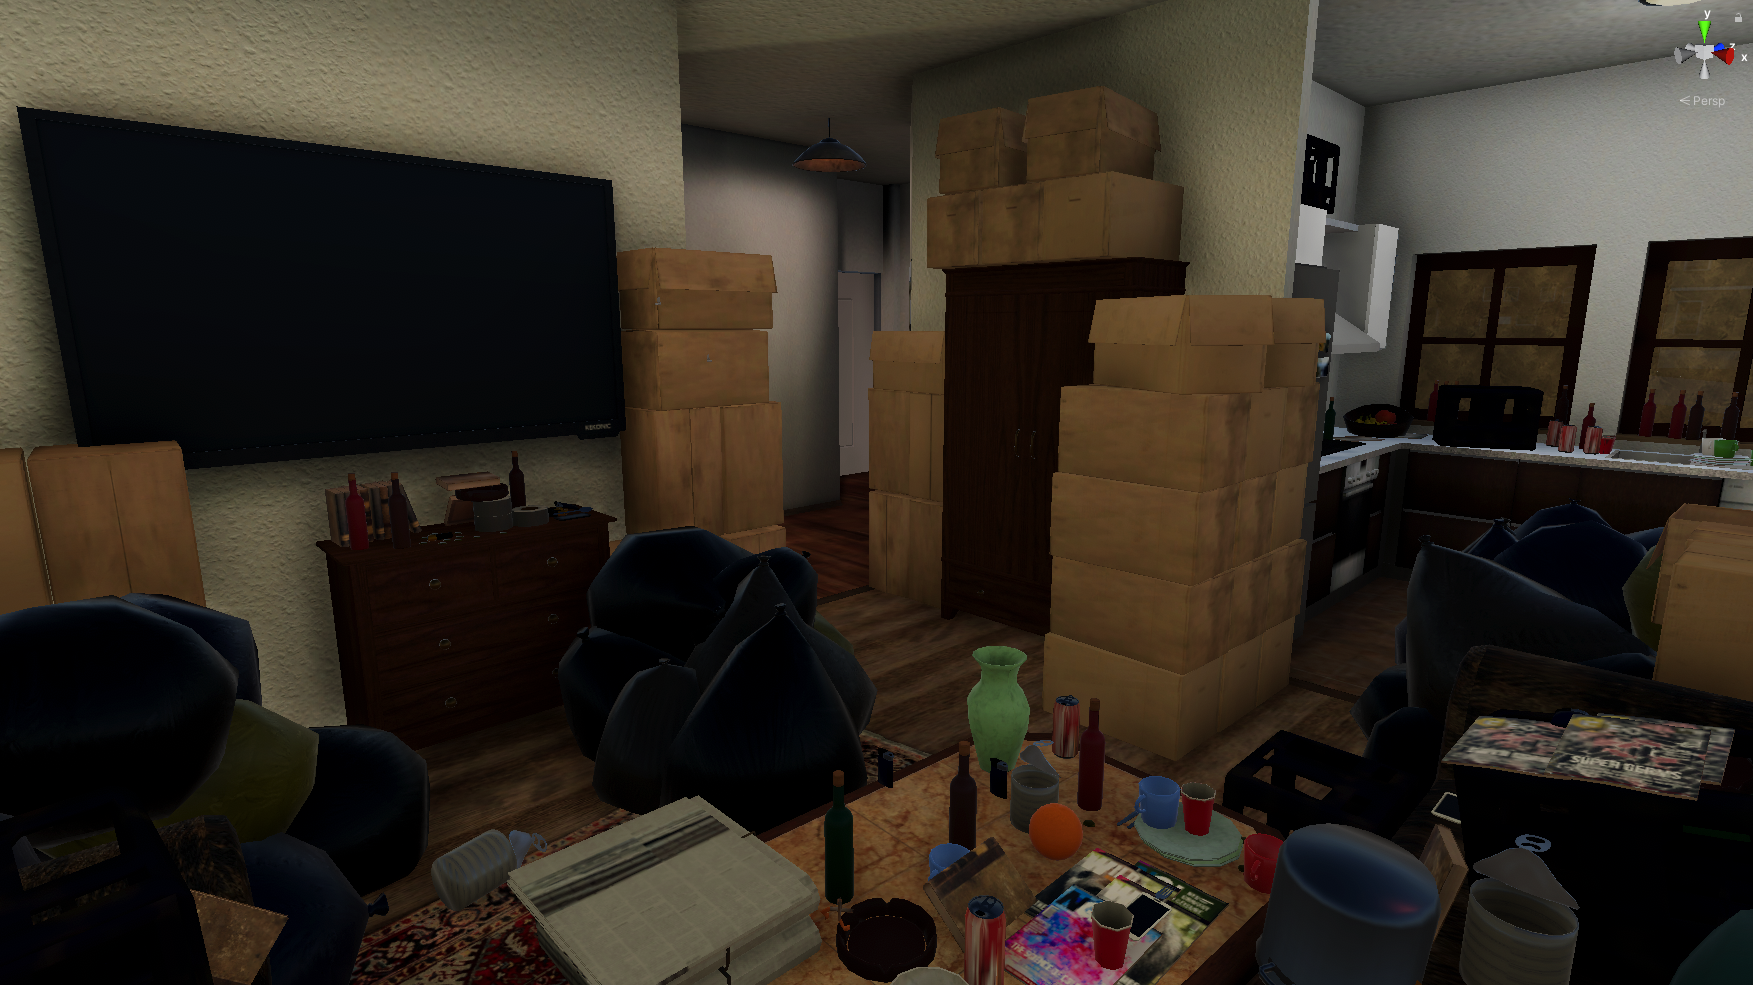
\includegraphics[width=0.7\textwidth]{Bilder/wohnzimmer Dunkel.PNG}
	\caption{An apartment which is illuminated in low key style. }
	\label{fig:darkroom}
\end{figure}
This effect is achieved by combining several techniques. Some of these will be discussed in more detail below. First, of course, the intensity of the lighting sources in the scene is adjusted. The sun in particular is a key light for the entire scene and has a very strong influence on the appearance of the apartment, which is why it is adjusted as a lighting source first of all. In addition to its intensity, the temperature of the color is also adjusted, and changed from a rather reddish tone to a bright, white and pleasant hue, making the scene generally look much brighter and much more details are visible. This represents the beginning of a transition to a high-key lighting style. 
\begin{figure}[H]
	\centering
		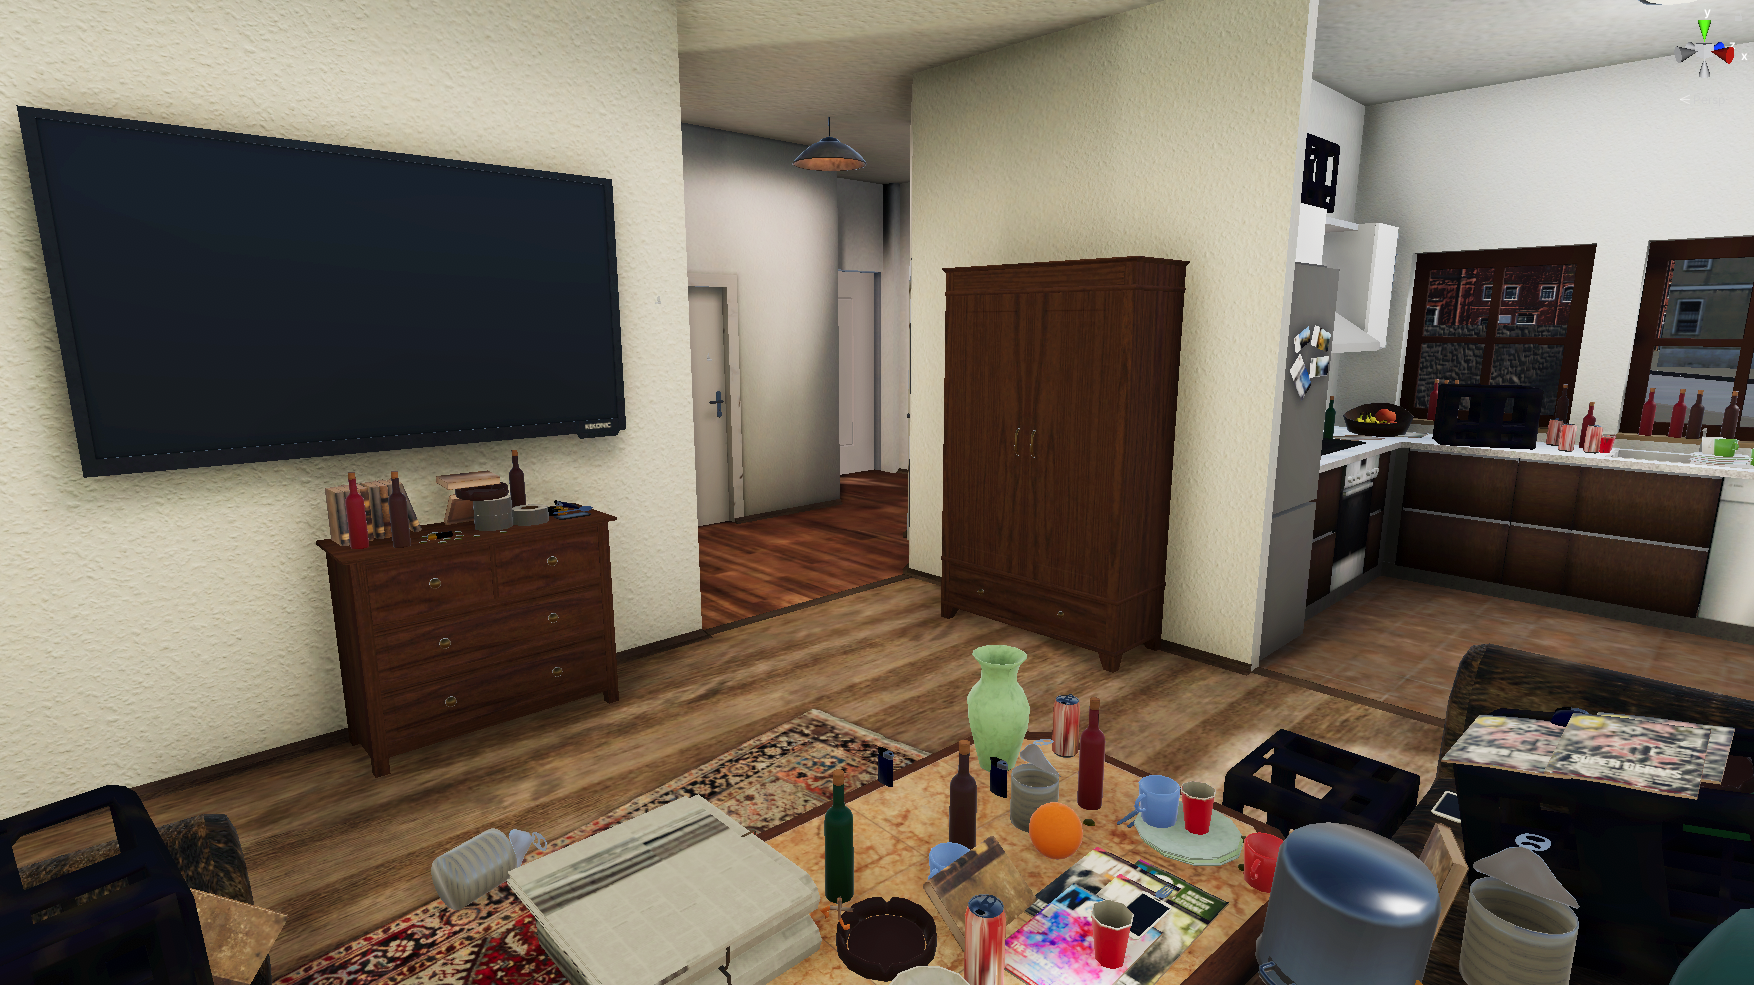
\includegraphics[width=0.7\textwidth]{Bilder/Wohnzimmer hell.PNG}
	\caption{The same apartment which is now illuminated in high key style. }
	\label{fig:darkroom}
\end{figure}
\newpage
In addition to the sun, the illuminance of the individual light sources in the apartment, i.e. ceiling lamps and floor lamps, is also adjusted and set much brighter. All of this contributes to making the scene much more enjoyable for the player. This gives him positive reinforcement, which should make him feel good every time he decides to throw an object in the trash. In addition, post-processing effects are also used. These effects ensure that the ambient light (previously also called fill light) is increased, making details of the scene much more recognizable. This can also be used as a further lever to confront the player with an increasingly better atmosphere.\\
The reason why all these efforts are made regarding the change of the light designg is, as briefly mentioned above, very simple: The more objects the player disposes of, the better and more pleasant the atmosphere of the virtual scene should become. The main reason for this is that it serves as a positive reinforcement for the patient (i.e. the player) and thus has a psychological benefit for the therapy of a messie-patient.\\
In general, an additional attempt is made to apply these effects and techniques slowly over a certain period of time. This not only leads to the generation of a visually more appealing image, but also to the fact that, in the best case, the patient only notices the change in the environment subconsciously and thus the desired illusion is maintained.
\\